
\documentclass[tikz,border=8pt]{standalone}
\usepackage{amsmath}
\usepackage{xcolor}
\usetikzlibrary{arrows.meta,positioning,calc,shapes.geometric}
\definecolor{Canvas}{HTML}{FAF9F6}
\definecolor{Ivory}{HTML}{FFFFF0}
\definecolor{Divider}{HTML}{E5E5EA}
\definecolor{Gold}{HTML}{C5A059}
\definecolor{WarmGold}{HTML}{D4AF37}
\definecolor{SoftPink}{HTML}{FBEFEF}
\definecolor{Ink}{HTML}{2C2C2E}
\tikzset{decision/.style={rectangle,draw=Gold,line width=1.2pt,fill=Canvas,minimum width=1.5cm,minimum height=1cm,align=center,text=Ink},chance/.style={circle,draw=WarmGold,line width=1.2pt,fill=Ivory,minimum size=1.45cm,align=center,text=Ink},payoff/.style={regular polygon,regular polygon sides=3,shape border rotate=90,draw=Gold,line width=1.2pt,fill=SoftPink,minimum size=1.25cm,align=center,text=Ink},branch/.style={draw=Ink,line width=0.9pt,-{Latex[length=2mm]},line cap=round},chosenbranch/.style={draw=Gold,line width=1.15pt,-{Latex[length=2mm]},line cap=round},callout/.style={rectangle,rounded corners=5pt,draw=Divider,fill=Ivory,text=Ink,align=center,inner sep=6pt}}

% Asset ID: OffSpecDecisionAnalysisTikZ-005
% Source: transcripts.md + ordinary A-Level Maths bridge
% Purpose: Compare probability trees with decision trees and warn against probabilities on decision branches.
\begin{document}
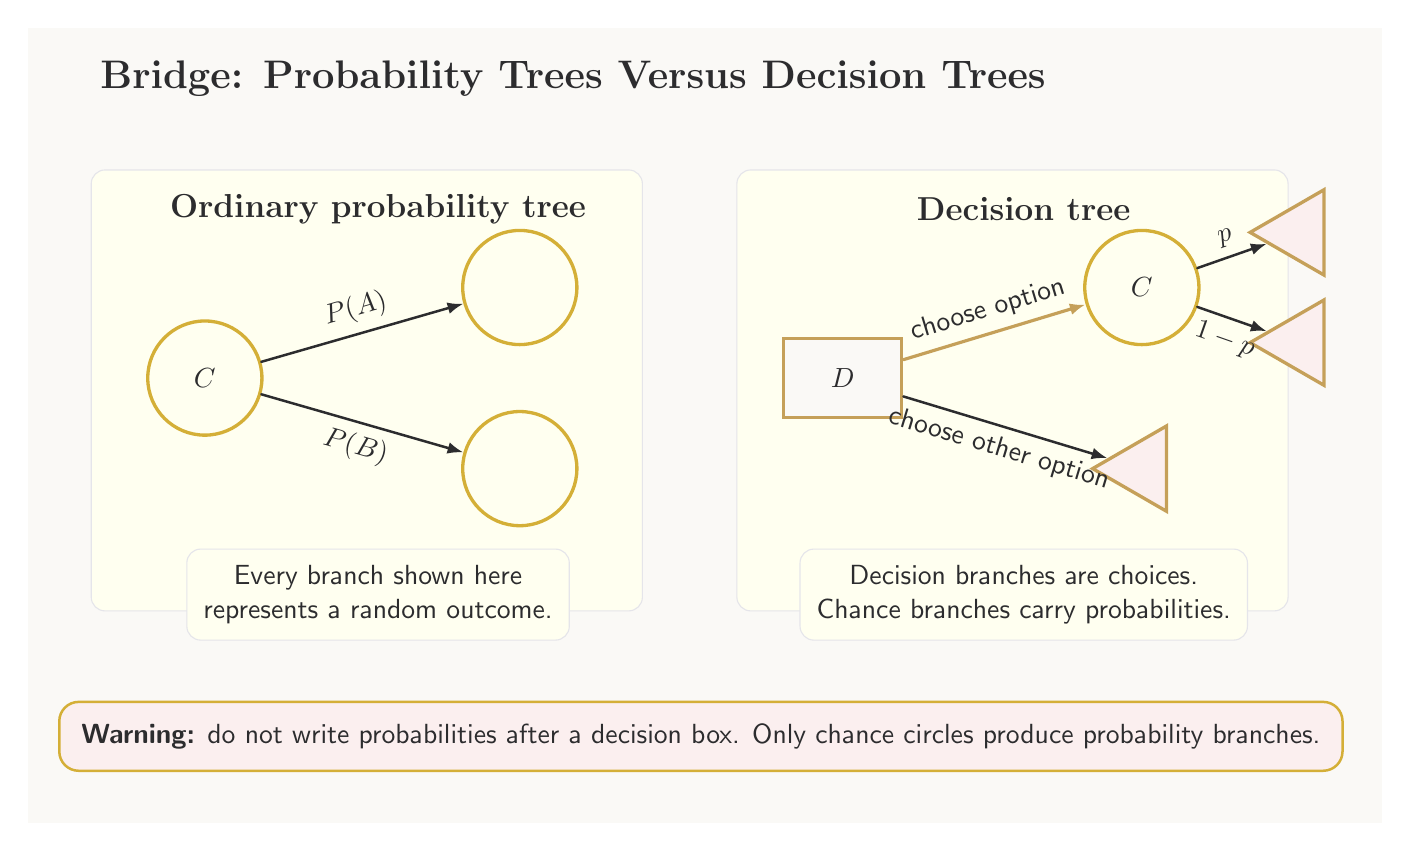
\begin{tikzpicture}[font=\sffamily,x=1cm,y=1cm]
\fill[Canvas] (-0.8,-1.55) rectangle (16.4,8.55);
\node[anchor=west,text=Ink,font=\bfseries\Large] at (0,7.9) {Bridge: Probability Trees Versus Decision Trees};
\node[callout,minimum width=7.0cm,minimum height=5.6cm,anchor=north west] at (0,6.75) {};\node[callout,minimum width=7.0cm,minimum height=5.6cm,anchor=north west] at (8.2,6.75) {};
\node[text=Ink,font=\bfseries\large] at (3.65,6.25) {Ordinary probability tree};\node[text=Ink,font=\bfseries\large] at (11.85,6.25) {Decision tree};
\node[chance] (P0) at (1.45,4.1) {$C$};\node[chance] (P1) at (5.45,5.25) {};\node[chance] (P2) at (5.45,2.95) {};\draw[branch] (P0)--node[above,sloped,text=Ink] {$P(A)$} (P1);\draw[branch] (P0)--node[below,sloped,text=Ink] {$P(B)$} (P2);\node[callout] at (3.65,1.35) {Every branch shown here\\represents a random outcome.};
\node[decision] (D0) at (9.55,4.1) {$D$};\node[chance] (D1) at (13.35,5.25) {$C$};\node[payoff] (D2) at (13.35,2.95) {};\draw[chosenbranch] (D0)--node[above,sloped,text=Ink] {choose option} (D1);\draw[branch] (D0)--node[below,sloped,text=Ink] {choose other option} (D2);\node[payoff] (D3) at (15.35,5.95) {};\node[payoff] (D4) at (15.35,4.55) {};\draw[branch] (D1)--node[above,sloped,text=Ink] {$p$} (D3);\draw[branch] (D1)--node[below,sloped,text=Ink] {$1-p$} (D4);\node[callout] at (11.85,1.35) {Decision branches are choices.\\Chance branches carry probabilities.};
\node[rectangle,rounded corners=7pt,draw=WarmGold,fill=SoftPink,line width=0.9pt,text=Ink,align=center,inner sep=8pt,minimum width=13.8cm] at (7.75,-0.45) {\textbf{Warning:} do not write probabilities after a decision box. Only chance circles produce probability branches.};
\end{tikzpicture}
\end{document}
